\section{Historical speculative decoding: separate evidence}
\label{sec:spec-history}

The latest native-AR matrix deliberately excludes DSpark. We retain the
September 11 full-target result as historical evidence, not a claim that the
latest merged DSpark service has been revalidated. This distinction also
prevents an earlier approximate-target speed from becoming a recovery target.

\subsection{Why the historical TP4 1.5k result is not a strict baseline}

In the old anchor-only/compact routed-MoE path, C32 with three draft positions
produced M128 target rows, but only 32 anchor rows executed the full routed
expert branch. Non-anchor rows omitted routed experts. Keeping stored weights
unchanged did not preserve the full target function at those positions.
Consequently, approximately 1.5k resident tok/s from that path is an
\emph{approximate-target} result. It cannot be presented as native AR or
lossless full-target verification, even if an early France answer passed.

M128 is a row count, not inherently speculative: native C128 would also
produce M128, whereas native C32 normally produces M32. Padding C32 to 128
does not compute three useful future AR positions for free. The new native
down-consumer pilot therefore tests actual M32 without reintroducing DSpark.

\subsection{Strict TP8 MHC fusion checkpoint}

The September 11 trial preserved all target experts, original weights,
TP-synchronized draft/accept decisions, a 1M logical pool, and gamma three.
It used 32 real-code requests, 512 outputs with \texttt{ignore\_eos}, and
chunk 2304. Four measured resident windows per family gave:

\begin{table*}[tp]
  \centering
  \caption{Historical full-target DSpark only; not a current AR comparison.
  Acceptance and throughput are reported in their original trial scope.}
  \label{tab:dspark-history}
  \begin{tabular}{@{}lrrr@{}}
    \toprule
    Family & Resident tok/s & Mean accept length & Relative to control \\
    \midrule
    Control & 1073.16 & 2.687 & --- \\
    Fusion + FP32 mixing & 1127.48 & 2.732 & +5.06\% \\
    Fusion + FP16 mixing & 1142.26 & 2.698 & +6.44\% \\
    \bottomrule
  \end{tabular}
\end{table*}

FP32 mixing was selected historically. The FP16--FP32 mean gap of about
1.31\% was smaller than the observed FP16-family range of 2.5\%, their ranges
overlapped, and only four windows per family were available. FP16 also had a
larger component perturbation and the trial's single observed semantic
degeneration. These observations motivate the conservative choice, not a
statistical proof that either rounding variant is universally safer.

\begin{figure*}[tp]
  \centering
  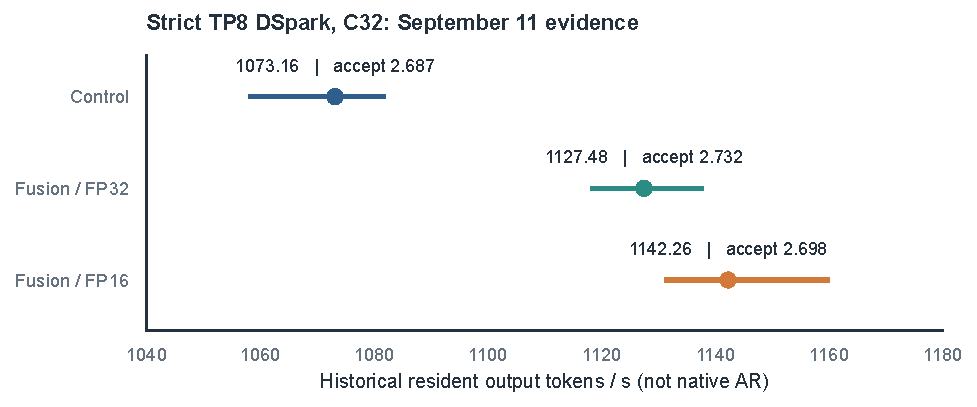
\includegraphics[width=.90\textwidth]{figures/strict_dspark_history.pdf}
  \caption{Historical strict DSpark family means with the ledger's rounded
  observed min/max ranges, not confidence intervals. Native AR, natural EOS,
  and the September 14 C32 pilot are deliberately not plotted on this axis.}
  \Description{Historical strict DSpark means are 1073.16 for control, 1127.48 for FP32 fusion, and 1142.26 for FP16 fusion; intervals are rounded observed ranges, not confidence intervals.}
\end{figure*}

\subsection{Acceptance, timing, and drift}

For concurrency $C$, average committed tokens per request $a$, and complete
speculative step time $T_{\mathrm{SD}}$, useful throughput is
$Ca/T_{\mathrm{SD}}$. It exceeds native AR only if
$T_{\mathrm{SD}}/T_{\mathrm{AR}}<a$. Larger verification batches expand expert
work and may not amortize draft cost. Acceptance alone is not a speed metric.

In the historical trial, chunked admission ramped the active batch through
several sizes before all requests were resident. Controls differed from
themselves on most complete output sequences. Such changes in batching and
numerical execution confound attribution from final hashes; they do not prove
that all other numerical or synchronization risks are absent. Most flagged
dot tails were forced continuation after EOS, distinct from genuine semantic
repetition. This motivated the natural-EOS protocol used in the new AR matrix.
The 1127.48 figure must not be divided by the new 1044.32 AR figure to claim a
matched speculative speedup: output policy, input mixture, chunking and date
differ. A fresh matched AR/strict-DSpark experiment remains outside this update.
